\documentclass{article}

% to do (5/16)

%% put more sparkles around writing OED in a program. Why is this clever and useful?

%% introduce max Entropy prior early (could also be interpolation between max ent and the predictive)
%%%% results of sequence prediction (formerly, "randomness") w.r.t. maxEnt vs. predictive (discuss why we think maxEnt is giving a better prediction here)

%% Figure 3 histogram: vertical line with AIG
%% create n_subjects analysis figure (a la FIgure 3, line plot) for sequence prediction... bootstrap up to n=100 to observe crossover


% if you need to pass options to natbib, use, e.g.:
% \PassOptionsToPackage{numbers, compress}{natbib}
% before loading nips_2016
%
% to avoid loading the natbib package, add option nonatbib:
\usepackage[nonatbib]{nips_2016}

%\usepackage{nips_2016}

% to compile a camera-ready version, add the [final] option, e.g.:
% \usepackage[final]{nips_2016}

\usepackage[utf8]{inputenc} % allow utf-8 input
\usepackage[T1]{fontenc}    % use 8-bit T1 fonts
%\usepackage{hyperref}       % hyperlinks
\usepackage{url}            % simple URL typesetting
\usepackage{booktabs}       % professional-quality tables
\usepackage{amsfonts}       % blackboard math symbols
\usepackage{nicefrac}       % compact symbols for 1/2, etc.
\usepackage{microtype}      % microtypography
\usepackage{amsmath}
\usepackage{mathtools}
\usepackage{fancyvrb}
\usepackage{multirow}
\usepackage{color}
\usepackage{textcomp}


% HT http://tex.stackexchange.com/a/151987/41154
\DeclarePairedDelimiterX{\infdivx}[2]{(}{)}{%
  #1\;\delimsize\|\;#2%
}
\newcommand{\dkl}{D_\mathrm{KL}\infdivx}

\usepackage{listings}
\definecolor{lightgray}{rgb}{.9,.9,.9}
\definecolor{darkgray}{rgb}{.4,.4,.4}
\definecolor{purple}{rgb}{0.65, 0.12, 0.82}
\definecolor{orange}{rgb}{1,0.5,0}

\definecolor{Red}{RGB}{255,0,0}
\newcommand{\red}[1]{\textcolor{Red}{#1}}
\definecolor{Green}{RGB}{10,200,100}
\definecolor{Blue}{RGB}{10,100,200}
\newcommand{\ndg}[1]{\textcolor{Green}{[ndg: #1]}}
\newcommand{\mht}[1]{\textcolor{Blue}{[mht: #1]}}
\newcommand{\lou}[1]{\textcolor{orange}{[lou: #1]}}

% casual outlining font
\newcommand{\cas}[1]{ \textsf{\color{darkgray} \scriptsize #1} }

\lstdefinelanguage{JavaScript}{
  keywords={typeof, new, true, false, catch, function, return, null, catch, switch, var, if, in, while, do, else, case, break},
  keywordstyle=\color{blue}\bfseries,
  ndkeywords={class, export, boolean, throw, implements, import, this},
  ndkeywordstyle=\color{darkgray}\bfseries,
  identifierstyle=\color{black},
  sensitive=false,
  comment=[l]{//},
  morecomment=[s]{/*}{*/},
  commentstyle=\color{purple}\ttfamily,
  stringstyle=\color{red}\ttfamily,
  morestring=[b]',
  morestring=[b]"
}

\lstset{
   language=JavaScript,
   backgroundcolor=\color{white},
   extendedchars=true,
   basicstyle=\footnotesize\ttfamily,
   showstringspaces=false,
   showspaces=false,
   numbers=none,
   numberstyle=\footnotesize,
   numbersep=9pt,
   tabsize=2,
   breaklines=true,
   showtabs=false,
   captionpos=b
}



\usepackage[ruled,vlined]{algorithm2e}

\newcommand{\ud}{\,\mathrm{d}}
\DeclareMathOperator*{\argmax}{arg\,max}


\title{Practical optimal experiment design with probabilistic programs}

% The \author macro works with any number of authors. There are two
% commands used to separate the names and addresses of multiple
% authors: \And and \AND.
%
% Using \And between authors leaves it to LaTeX to determine where to
% break the lines. Using \AND forces a line break at that point. So,
% if LaTeX puts 3 of 4 authors names on the first line, and the last
% on the second line, try using \AND instead of \And before the third
% author name.

\author{
  David S.~Hippocampus\thanks{Use footnote for providing further
    information about author (webpage, alternative
    address)---\emph{not} for acknowledging funding agencies.} \\
  Department of Computer Science\\
  Cranberry-Lemon University\\
  Pittsburgh, PA 15213 \\
  \texttt{hippo@cs.cranberry-lemon.edu} \\
  %% examples of more authors
  %% \And
  %% Coauthor \\
  %% Affiliation \\
  %% Address \\
  %% \texttt{email} \\
  %% \AND
  %% Coauthor \\
  %% Affiliation \\
  %% Address \\
  %% \texttt{email} \\
  %% \And
  %% Coauthor \\
  %% Affiliation \\
  %% Address \\
  %% \texttt{email} \\
  %% \And
  %% Coauthor \\
  %% Affiliation \\
  %% Address \\
  %% \texttt{email} \\
}

\begin{document}
% \nipsfinalcopy is no longer used

\maketitle

\begin{abstract}

Designing good scientific experiments requires ingenuity, rigor, and patience to consider a large space of possible experiments.
With the growing popularity of formal models, part of this time-consuming process can be automated.
Here, we present a general and principled approach to experiment design.
Our system is based on a user-friendly probabilistic programming language (PPL).
Using such a high-level and universal modeling language means details of experiment selection calculation can be hidden from the scientist, without loss of generality; she needs only represent her hypothesis and space of potential experiments.
We apply this system to differentiating competing models of psychological phenomena, but the framework is general to any domain where probabilistic models are used to represent theories.
We validate our framework using case studies in the psychology of randomness and categorization.
We find strong empirical validation that our automatically designed optimal experiments were indeed optimal.
Our framework opens up a number of interesting questions, which we explore in the discussion.


\end{abstract}

%\mht{I think in practice ``the space of possible experiments'' is the same thing as an ``empirical paradigm''. This terminology may be useful in our exposition.}

\section{Introduction}
%\lou{start off more generally, don't specialize too much for psychology.}
%\ndg{agree: first talk about OED in general, and why we should do OED within a PPL setup, then talk about psych as a target domain.}
Designing scientific experiments is hard.
Scientists must have hypotheses and reason over a potentially large space of possible experiments.
Formal models alleviate some of these issues.
Models make explicit hypotheses about observed data, and thus make it easier (or in some cases, possible) to explore the implications of a set of theoretical ideas.
However, exploring models can be time-consuming and searching through a large space of possible experiments is still largely driven by the scientist's intuition.
This intuition may be biased towards experiments that show qualitative differences between models, even when they are not very informative.
%\ndg{point out that this intuition can be wrong -- foreshadow MS result...}
This need not be the case: If both the set of hypotheses and the space of experiments are explicit, then we can partially \emph{automate} experiment design as a sort of active learning problem, searching for experiments that maximally update our beliefs about a scientific question.

We present a general and principled framework for experiment design that uses a Bayesian approach to find experiments that best distinguish competing hypotheses.
For such a framework to be domain-general, the computation for experiment selection must be automatic.
This is only possible with a common formalism for specifying hypotheses and experiments.
\emph{Probabilistic programming languages} (PPLs) are such a formalism; they are high-level and universal languages for expressing probabilistic models.
This is a crucial step in making a practical OED system: Once you're using a PPL to formalize your hypotheses, OED comes for free.

We first describe our framework in general terms and then apply it in two case studies from cognitive psychology, a field where experiments have certain challenging features: human participants give noisy responses, experimental results are sensitive to sample size, and computational models often do not make direct predictions about experimental data, instead requiring \emph{linking functions}.
In the first case study, we consider the problem of disambiguating three toy models of perceptions of subjective randomness.
In the second case study, we go beyond toy models and analyze a classic paper on human categorization learning that compared two models using an experiment designed by hand; we find that OED discovers experiments that are more effective in an information-theoretic sense.
Our general system opens a number of rich areas for future development, which we explore in the discussion.

%We conclude by highlighting the generality of the approach and areas of future work.
%\ndg{all the parts are here. needs smoothing. make it clearer that using PPL to represent hypotheses is a key step in making the system practical.}

%    \begin{itemize}
%        \item It is difficult to discriminate models of psychological processes
%        \item Experiments are expensive
%        \item We present a general, turn-key approach to design experiments that best disambiguate competing models using a Bayesian framework
%        \item This technique is not directly related to Bayesian models of cognition. It can be used on any (formal / probabilistic) model, including Bayesian models of cognition
%        \item Despite the previous attempts in this field, there are a number of pragmatic issues that make it difficult to readily apply OED techniques for psychology, including:
%        \begin{itemize}
%            \item A variety of proposed optimization criteria, which puts the burden on researchers to have sufficient expertise to select the appropriate approach
%            \item A lack of an established pipeline, requiring researchers to develop a language to formalize psychological models and write an OED optimization engine
%            \item A lack of analysis in dealing with practical experimental concerns such as:
%                \begin{itemize}
%                    \item Noisy responses from participants
%                    \item The ideal number of participants for a study
%                    \item The ambiguity of linking functions of dependent measures
%                \end{itemize}
%        \end{itemize}
%    \end{itemize}


\section{Experiment design framework}
\label{s:bayes}

Let us put on our scientist hats---we wish to compare a set of models $M$ in terms of how well they account for empirical phenomena.
A model $m$ is a conditional distribution $P_m(Y \mid X)$ representing the likelihood of empirical results $y$ for different possible experiments $x$ (we also write $m(x)$ as shorthand for $P_m(Y \mid X = x)$).
We begin with a prior belief distribution $P(M)$ and aim to conduct an experiment $x$ that maximally updates this distribution.
Formally, we wish to find
$$x^{*} = \argmax_{x} \dkl{ P(M \mid X = x) }{ P(M) }.$$
\emph{A priori}, we do not know what the result of any particular experiment will be, so we must integrate over the possible results $y$:
\begin{align}
  x^{*} &= \argmax_{x} \sum\limits_{y}p(y ; x) \dkl{ P(M \mid X = x, Y = y) }{ P(M) }  \label{eq:oed}
\end{align}
where $p(y ; x)$ is the probability of observing result $y$ for experiment $x$.
If we have reason to believe that $M$ contains the true model of the data, then a suitable choice for $p(y ; x)$ is the predictive distribution implied by the models $ \sum\limits_{m}p_m(y \mid x)p(m) $.
If, however, we do not believe that $M$ contains the true model, then an uninformative prior $p(y ; x) \propto 1$ may be more appropriate.

Consider a concrete example.
Imagine that we are studying how people predict values for sequence data (e.g., coin flips) and we want to compare two models: $m_{\text{fair}}$, in which people believe the coin is unbiased, and $m_{\text{bias}}$, in which people believe the coin has an unknown bias (a uniform prior on the unit interval) that can be learned from data.
We have a uniform prior on the models but we wish to update this belief distribution by conducting an experiment where we show people 4 coin flips and ask them to predict the next one.
So there are 16 possible experiments and $2^n$ possible responses---heads or tails for each of $n$ human participants.
Each model is thus a probability distribution on $\{0,1\}^n$ conditional on the experiment $x$.
For convenience, we write our models $m_{\text{fair}}$ and $m_{\text{bias}}$ in terms of a what a single person would do and assume that all people use this same model, i.e., participant responses are IID.\footnote{We use this simple linking function throughout this paper but our approach handles arbitrary linking functions (e.g., hierarchical models).}

How informative would running the experiment, say, \lstinline{HHTT} be?
$m_{\text{fair}}$ and $m_{\text{bias}}$ are identical here (heads and tails are equally likely)---neither experimental result would change our belief in one of the models, so this is a poor experiment.
By contrast, the experiment \lstinline{HHHH} would be much more informative.
Under $m_{\text{fair}}$, $p(\texttt{H}) = \frac{1}{2}$ but under $m_{\text{bias}}$ $p(\texttt{H}) = \frac{5}{6}$.
If we ran our experiment with a single participant, \emph{either} empirical response would be informative.
If the participant predicted heads, this would favor $m_{\text{bias}}$ and if she predicted tails, this would favor $m_{\text{fair}}$.
Thus, \lstinline{HHHH} would be a good experiment to run.
In what follows, we show how to automate this sort of reasoning.

\subsection{Writing models as probabilistic programs}

A key requirement for automating experiment design is to write models of the data as programs---in our case, probabilistic programs.
We use the probabilistic programming language WebPPL (\url{webppl.org}), a small but feature-rich probabilistic programming language embedded in Javascript \cite{dippl}.
WebPPL supplies a number of primitive distributions (e.g. \lstinline{Binomial}), which  support generating samples and calculating the density of values.
For instance, we can sample from $\text{Binomial}(4, \frac{1}{2}$ using \lstinline|sample(Binomial({n: 4, p: 0.5}))| and we can determine the log-probability of the value 2 under this distribution using \lstinline|score(Binomial({n: 4, p: 0.5}), 2)|.

Oftentimes, we are interested in posterior inference. Let's say we are interested in the Binomial(4, 0.5) distribution conditional on at least 2 successes. We write this as:
%
\begin{lstlisting}[mathescape, label={code:webppl}, caption = {Posterior inference in WebPPL.}]
var conditionalBinomial = function(){
	var x = sample(Binomial({n: 4, p: 0.5}))
	condition(x >= 2)
	return x
}
\end{lstlisting}

In Listing \ref{code:webppl}, \lstinline{conditionalBinomial} represents a sampler for the conditional distribution---we draw a sample \lstinline{x} from the prior, reject values less than 2 using \lstinline{condition}, which enforces hard constraints (an alternate form called \lstinline{factor} is used for soft constraints), and return \lstinline{x}.
\lstinline{conditionalBinomial} is a declarative specification of the model we would like to sample from.
To actually obtain samples, we must perform inference on this model using \lstinline{Infer(model, options)}.
This provides a useful separation for the scientist--we distinguish \emph{what} we would like to compute from \emph{how} we try to compute it.
WebPPL currently provides several inference algorithms to choose from: MCMC (Metropolis-Hasting, Hamilton Monte Carlo), full enumeration for discrete models, Sequential Monte Carlo, and variational inference.

\subsection{Writing OED as a probabilistic program}

Surprisingly, because we have expressed the space of models, experiments, and responses in the language of probability, it is also straightforward to express OED as a probabilistic program (see Listing \ref{code:oed-pp}).
Equation~\ref{eq:oed} translates to around 20 lines of WebPPL code that makes it clear that OED is an inference problem.
Expressing OED in this way gives us access to algorithms that are more sophisticated than previous research has considered  (e.g., mixtures of Enumeration and HMC for  experiment spaces that have continuous and discrete subspaces).

Note that we implement search for the optimal experiment using inference.
This is not essential---we could also replace the outermost \lstinline|Infer()| call with an optimization procedure (e.g., \lstinline|Search()|).

%\begin{minipage}{\linewidth}
\begin{lstlisting}[mathescape, label={code:oed-pp}, caption = {OED implementation. For clarity, we have omitted some book-keeping details.}]
var OED = function(mSample, xSample, ySample) {
  var mPrior = Infer(function() { mSample() })
  Infer(function() {
    var x = xSample();
    var KLDist = Infer(function() {
      var y = ySample()                   // ${\color{purple} p(y ; x)}$
      var mPosterior = Infer(function() { // ${\color{purple} \dkl{ P(M \mid Y = y) }{ P(M) } }$
        var m = sample(mPrior)
        factor(score(m(x), y))
        return m.name
      })
      return KL(mPosterior, mPrior)
    })
    var EIG = expectation(KLDist)  // ${\color{purple} \sum_{y} p(y ; x) \dkl{ P(M \mid Y = y) }{ P(M) } }$
    factor(Math.log(EIG / maxEIG)) // optional (inference as search)
    return {x: x, EIG: EIG}
  })
}
\end{lstlisting}
%\end{minipage}
Our OED code is available as a WebPPL package---see \url{https://github.com/mhtess/webppl-oed}.
We next illustrate our system by applying it to distinguish psychological theories of sequence prediction.

\section{Case study 1: Sequence prediction}
\label{s:tutorial}

Human judgments about sequences are surprisingly systematic and nonuniform across equally likely outcomes -- for example, we might strongly the next flip in the  sequence of coin flips \lstinline{HHTTHHTT} will be \lstinline{H}, whereas we might assign equal probability of \lstinline{H} and \lstinline{T} for the sequence \lstinline{THHTHTHT}.
There are many hypotheses one might have about what underlies human intuitions such sequences.
Here, we consider three simple hypotheses about the beliefs that participants have about the coin flips\footnote{These are computational-level models of a \emph{person's model} of the situation. For more details on this kind of cognitive modeling, see \url{https://probmods.org}}: (a) \emph{Fair coin}: participants assume the coin is fair, (b) \emph{Bias coin}: participants believe the coin has some unknown bias (i.e., the probability of a \lstinline{H} outcome) that they can learn from data, (c) \emph{Markov coin}: participants believe the coin has some probability of transitioning between spans of \lstinline{H} and \lstinline{T} outcomes.
We consider an experimental setup where participants observe four flips of the same coin and are asked to predict the outcome of the next flip.


\subsection{Formalization}

Formally, the model space $M$ is $\{m_{\text{fair}}, m_{\text{bias}}, m_{\text{markov}}\}$, the experiment space $X$ is the set of all possible sequences of four coin flips, and the set of responses $Y$ is a choice between heads or tails for the fifth flip.

In $m_{\text{fair}}$, we model participants as believing that the coin has an equal probability of coming up heads or tails:

\begin{lstlisting}[caption=Fair coin model,  label={lst:m_fair},upquote=true]
  var fairCoin = function(seq) {
    Infer(function(){
      return flip(0.5)
    }, {method: 'Enumerate'})
  }
\end{lstlisting}

Note the type signature of this model -- it takes as input an experiment and returns a distribution on possible responses for the measurement of that experiment.
This distribution is computed using a particular inference strategy, here, an exhaustive \lstinline{Enumerate} algorithm.
$m_{\text{bias}}$ generalizes this fair coin model---people assume the coin has some unknown bias, learn it from observations, and use it to predict the next coin flip:

\begin{lstlisting}[caption=Biased coin model,  label={lst:m_weighted}, upquote=true]
var coinWeights = [0.01,0.1,0.2,0.3,0.4,0.5,0.6,0.7,0.8,0.9,0.99]
var biasCoin = function(seq) {
  Infer(function(){
    var bias = uniformDraw(coinWeights)
    var flipCoin = function(){ return flip(bias) }
    var sampledSeq = repeat(seq.length, flipCoin)
    condition(arrayEquals(seq,sampledSeq))
    return flipCoin()
  }, {method: 'Enumerate'})
}
\end{lstlisting}

$m_{\text{bias}}$ first samples a coin weight \lstinline{bias} from a discretized uniform distribution, and
then creates a helper function \lstinline{flipCoin} which samples observation from the weighted coin.
The model then generates a sequence of coin flips the same length as the observed sequence \lstinline{repeat(seq.length, flipCoin)} and conditions on this matching the observed sequence \lstinline{seq}.
The model then returns the outcome of the next coin flip.

Finally, $m_{\text{markov}}$ assumes that the coin is generated by a Markov process where the first coin flip is uniform and subsequent flips have some probability of transitioning away from the previous value.
The probability of transitioning from the current coin flip is inferred from the data, and is then used to predict the next flip:

\begin{lstlisting}[caption=Markov coin model, upquote=true]
var markovCoin = function(seq) {
  Infer(function(){
    var transProb = uniformDraw(coinWeights)
    var sampleOne = function(lastFlip) {
        return flip(transProb) ? !lastFlip : lastFlip
    }
 	  var sampleSeq = function(flipsSoFar, n) {
      if (n == 0) {
        return flipsSoFar
      } else {
        var nextFlip = sampleOne(last(flipsSoFar))
        return sampleSequence(append(flipsSoFar, nextFlip),
                              n - 1)
      }
    }
	  var sampledSeq = sampleSeq([flip(0.5)], seq.length - 1)
    condition(arrayEquals(seq, sampledSeq));
    return sampleOne(last(sampledSeq))
  }, {method: 'Enumerate'})
}
\end{lstlisting}

\subsection{Predictions of optimal experiment design}

Using an uninformative prior for $p(y; x)$, we ran OED for three model comparison scenarios: fair--bias, bias--Markov, and fair--bias--Markov (Fig.~\ref{fig:run-coin}).

\begin{figure}[h]
\underline{\textsf{(Example) Input:}}
\begin{lstlisting}
OED({mSample: function() { uniformDraw([fairCoin, biasCoin]) }),
     xSample: function() { repeat(4, flip) }, // experiment space
     ySample: function() { flip() })          // response space
\end{lstlisting}

\underline{\textsf{Output:}}\\
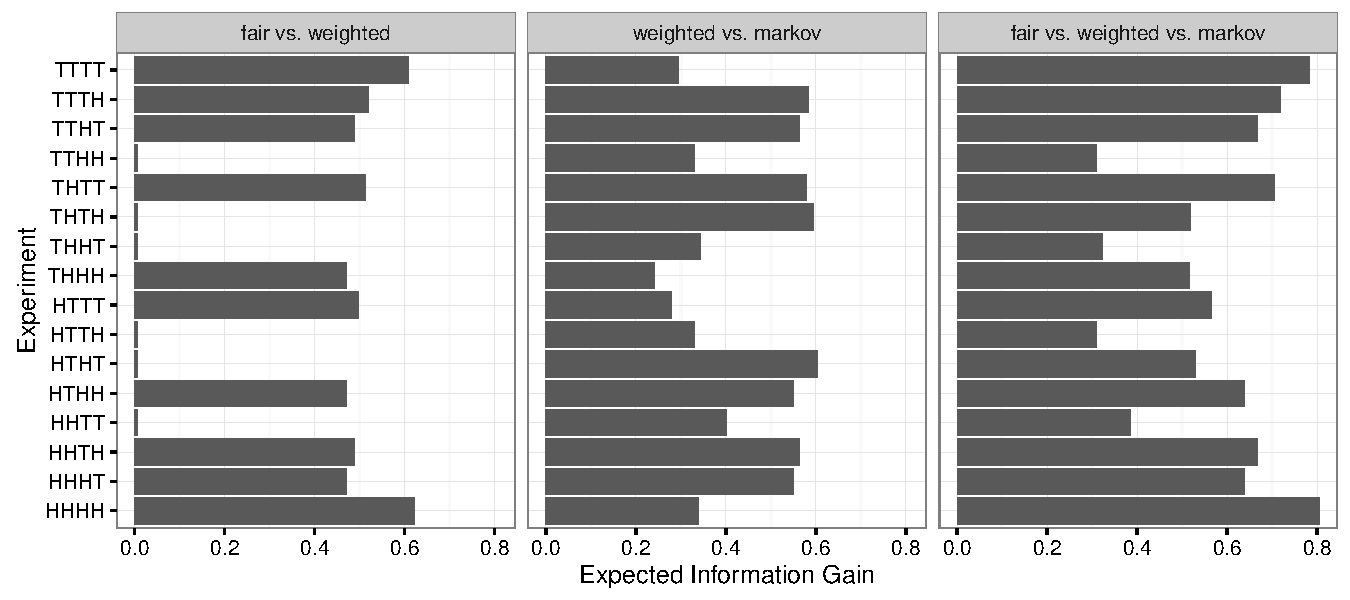
\includegraphics[width=\columnwidth]{img/coin_eig.pdf}
\caption{Running OED in the subjective randomness domain \mht{this is with the number of subjects that we collected; might want to make this for n = 1 (or n = 20) to highlight the symmetries}} \mht{Note this is also with the ignorance prior}
%\lou{make this figure in ggplot, clean it up}
\label{fig:run-coin}
\end{figure}
Consider the fair--bias comparison.
Observe that there are several experiments that have 0 information gain (e.g., \lstinline{TTHH}).
This is intuitive---the models make exactly the same predictions in this case, so the experiment has no distinguishing power.
The most informative experiments are \lstinline{HHHH} and \lstinline{TTTT}.
This is also intuitive---the bias model would infer a strongly biased coin and make a strong prediction, while the fair coin model is unaffected by the observed sequence.

Next, consider the bias--Markov comparison.
\lstinline{HHHH} and \lstinline{TTTT} are the least informative experiments---similar to fair--bias comparison, the models make similar predictions for these experiments.
\lstinline{HTHT} and \lstinline{THTH} are the most informative experiments.
This makes sense---the bias model infers a 0.5 probability of heads and so assigns equal probability of heads and tails to the next flip, whereas the Markov model infers that the probability of transitioning is high and assigns high probability to the opposite of the last observed value (\lstinline{T} for \lstinline{THTH} and \lstinline{H} for \lstinline{HTHT}).

Finally, consider the fair--bias--Markov comparison.
The worst experiments, \lstinline{TTHH}, \lstinline{THHT}, \lstinline{HTTH}, and \lstinline{HHTT}, are cases where all models make similar predictions.
The best experiments are \lstinline{TTTT} and \lstinline{HHHH}.
This result is less intuitive, which reveals the utility of an automated tool for experiment design.

%Finally, the expected information gain of experiments designed to disambiguate all three models is more complex to understand.
%The information gain now depends on how well the experiments disambiguate all three models. Here, we see that for


\subsection{Empirical validation}
We validated our OED system by running all of 16 experiments and comparing expected information gain with the actual information gain from empirical results.
We recruited 330 participants from Amazon's Mechanical Turk and randomly assigned each participant to a single experiment (all of the 16 experiments were completed by $\geq$20 unique participants).
Participants pressed a key to sequentially reveal the sequence of 4 flips and then made a prediction about the of the next coin flip (either heads or tails).

For each experiment $x$ and result $y$, we computed the expected information gain from running 20 participants\footnote{because we do client-side randomization, N's are not actually 20; we use the empirical N's for EIG} and compared this to the actual information gain, $\dkl{P(M \mid Y = y, X = x)}{P(M)}$, for the three model comparison scenarios.
Figure \ref{fig:aig_vs_eig} shows that expected information gain is a reliable predictor of the empirical value of an experiment (minimum $r$ = 0.857).

\begin{figure}[t]
\centering
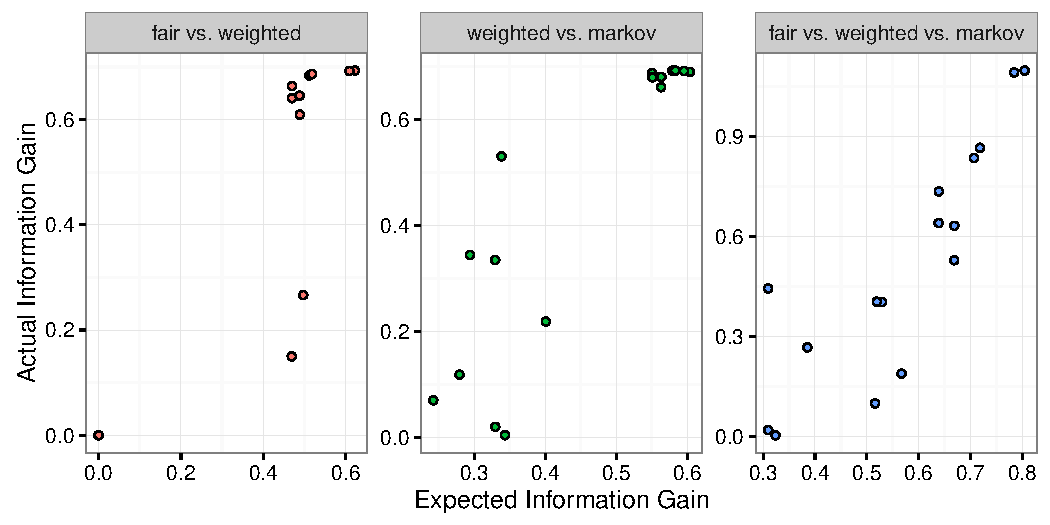
\includegraphics[width=0.7\columnwidth]{img/coin_eig_aig_scatter_noText.pdf}
\caption{Actual vs. expected information gain for three model comparison setups.}
\label{fig:aig_vs_eig}
\end{figure}

\section{Case study 2: Category learning}

Here, we explore a more complex and realistic space of models and experiments.
In particular, we analyze a classic paper in the psychology of categorization by Medin and Schaffer \cite{medin78:pr} that aimed to distinguish two competing models of category learning -- the \emph{exemplar model} and the \emph{prototype model}.
Using intuition, Medin and Schaffer (MS) designed an experiment where the models made diverging predictions and found that the empirical data from this experiment supported the exemplar model.
Subsequently, many other authors followed their lead, replicating and using this experiment to test competing models.

Here, we ask: how good was the MS experiment?
Could they have run an experiment that was more information-theoretically efficient?
Using our OED framework, we find that there are many superior experiments that Medin and Schaffer could have designed but did not.\footnote{Our work here is an exercise in counterfactual history; the Medin and Schaffer models are not state of the art. We chose the Medin and Schaffer research (rather than newer work) as an object of study because it commits to a clear set of competing models and a clear set of possible experiments.}



\subsection{Models}

Both the exemplar and prototypes model are classifiers that map inputs (objects represented as a vector of Boolean features) to a probability distribution on the categorization response (a label: A or B).
The exemplar model assumes people store information about every instance of the category they have observed; categorizing an object is thus a function of the object's similarity to all of the examples of category A versus the similarity to all of B's examples.
By contrast, the prototype model assumes assumes that people store a measure of central tendency for each category---a prototype.
Categorization of an object is thus a function of its similarity to A prototype  A versus its similarity to the B prototype.
For details, see the supplement.

\subsection{Experiments}

Participants first learn about the category structures in a training phase where they perform supervised learning of a subset of the objects and are then tested on this learning in a test phase.
During training, participants see a subset of the objects presented one at a time and must label each object.
Initially, they can only guess at the labels, but they receive feedback so that they can eventually learn the category assignments.
After reaching a learning criterion, they complete the test phase, where they label all the objects (training set and the held out test set) without feedback.

Medin and Schaffer used visual stimuli that varied on 4 binary dimensions (color: \emph{red} vs. \emph{green}, shape: \emph{triangle} vs. \emph{circle}, size: \emph{small} vs. \emph{large}, and count: \emph{1} vs. \emph{2}).
For technical reasons, they considered only experiments (1) having linearly separable decision boundaries and (2) containing 5 A's and 4 B's in the training set.
There are, up to permutation, 933 experiments that satisfy these constraints.
%This space is roughly two orders of magnitude larger than the space of subjective randomness experiments we considered before, although it is small enough to fully enumerate in a reasonable amount of time.

\subsection{Predictions of optimal experimental design}

Using the predictive prior for $p(y; x)$, we computed the expected information gain for all 933 experiments and found that the best experiment (for a single participant) had an expected information gain of 0.08 nats, whereas the MS experiment had an expected information gain of only 0.03 nats; thus, the optimal experiment is expected to be 2.5 times more informative than the MS experiment.
Indeed, the MS experiment ranks 665th out of 993 experiments total (Figure~\ref{fig:dist}a) \lou{rerun this with unconditioned prior}.

Why is the MS experiment ineffcient?
One reason is that Medin and Schaffer prioritized experiments that predict a qualitative categorization difference (i.e., if an object is predicted to be an A by one model but a B by the other).
The experiment they designed indeed predicts a qualitative difference, but this has a small magnitude and comes at the expense of little information gain from the remaining stimuli.
The optimal experiment is better able to quantitatively disambiguate the models by maximizing the information from all the stimuli simultaneously.

\begin{figure}[t]
\centering
\begin{tabular}{l l}
(a) & (b)\\
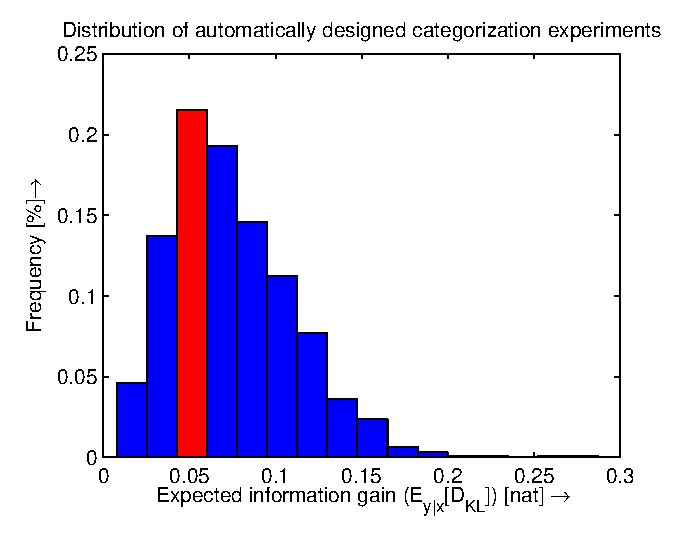
\includegraphics[width=2.5in]{img/dist.eps} & 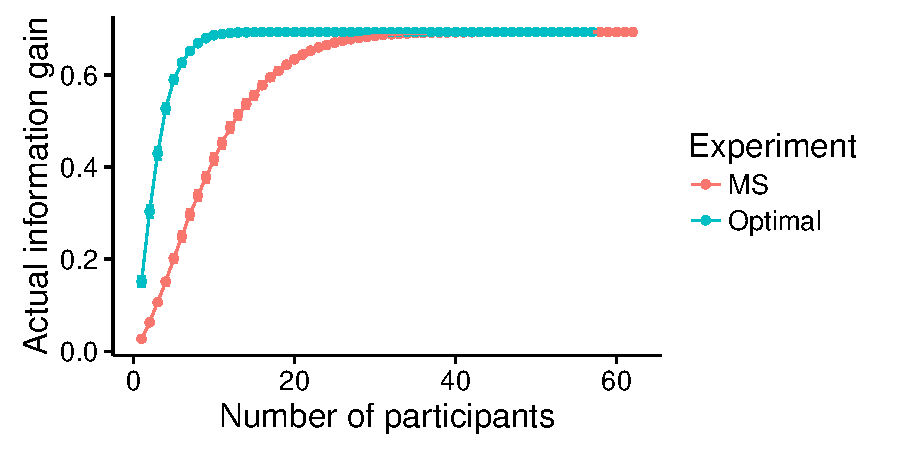
\includegraphics[width=2.5in]{img/category-ns.pdf}\\
\end{tabular}
\caption{Comparing MS and optimal experiments. MS experiment has lower expected information gain and requires three times as many participants to achieve maximum actual information gain.}
\label{fig:dist}
\end{figure}

\subsection{Empirical validation}

To validate our expected information gain calculations, we ran the MS and optimal experiments with 60 participants each.
Figure~\ref{fig:dist}b shows that both experiments achieve maximal actual information gain but the optimal experiment takes only 10 participants to asymptote to this maximum, whereas the MS experiment takes around 30.
Thus, the optimal experiment provides the same amount of information for 1/3 the experimental cost.

% and illustrates how automated experiment design can outperform human intuition. In particular, this case study demonstrates the efficacy of OED in psychology for discrete and non-ordinal experiment spaces, large combinatoric experiment spaces, and parametric model classes.

\section{Related work}

In our reading of the literature, we found that the basic intuition behind OED---to find experiments that maximize some expected measure of informativeness---has been independently discovered in a number of fields, including physics (berg03), chemistry (huan10), biology (vanlier12, liepe13), psychology (myung09), statistics (lindley72), and machine learning (golovin10).

These papers, however, often implement OED in a one-off fashion, specializing for  particular models (e.g., in biology: parameter estimation for ordinary differential equations with Gaussian noise) and commiting to a single inference technique (e.g., Metropolis-Hastings).
By contrast, we show that OED can be expressed as a generic, concise, and flexible function in a probabilistic programming language, which allows practitioners to rapidly explore different spaces of models, experiments, and inference algorithms.
Additionally, our work is the first to (1) demonstrate that expected information gain is a reliable predictor of actual information gain and to (2) characterize the cost benefits of OED.

\section{Conclusion}

Practitioners aim to design experiments that yield informative results.
Our approach partially automates experiment design, searching for experiments that maximally update beliefs about the model distribution.
With our approach, the scientist writes her hypotheses as probabilistic programs, sketches a space of possible experiments, and turns the crank of Bayesian inference.
We stress that our work \emph{complements} practitioners; it does not replace them.
Our tool eliminates the need to manually comb large spaces in search of good experiments; we hope that this will free scientists and engineers to work on the more interesting problems---devising empirical paradigms and building models.

We close by outlining some interesting directions for future work.
First, we chose KL divergence between posterior and prior as our informativeness measure because it is a well-known divergence function, but other choices (e.g., TV distance) might also be suitable.
Second, there might exist inference techniques that take advantage of the particular structure of the OED problem (e.g., it may be acceptable to have a less precise estimate of information gain when $p(y)$ is negligible).
Third, we have restricted attention to ``one-shot'' experiments, but it would be interesting to extend our work to sequential settings (e.g., adaptive tests).
Fourth, we have ignored the cost of experiments, but it would be worth explicitly taking this into account.
Our informativeness approach could be usefully integrated with multi-objective optimization methods for real-world applications (e.g., MRI studies of rare patient populations, expensive aerospace experiments).
Finally, we showed case studies of our method in in cognitive psychology but we believe that it is broadly useful, so we invite practitioners to test our method.

\bibliographystyle{ieeetr}
\bibliography{oed_nips_2016}

\end{document}
